\section{DESENVOLVIMENTO}

\subsection{MATERIAIS}
	Este capítulo tem a finalidade de apresentar as tecnologias utilizadas.
	
\subsubsection{Python}
	Lançada por Guido Van Rossum em 1991, Python é uma linguagem de programação dinâmica, interpretada, robusta, multiplataforma e multiparadigma. Seus objetivos eram produtividade e legibilidade. Foi utilizada como linguagem de programação deste projeto.
	
\subsubsection{NumPy}
	NumPy é uma biblioteca para linguagem Python que contém vetores e matrizes de N dimensões além de fornecer um grande conjunto de funções e operações matemáticas. Foi utilizada neste projeto para facilitar o uso de operações matemáticas e como dependência do Matplotlib.
	
\subsubsection{Pandas}
	Pandas é uma biblioteca para linguagem Python para trabalhar com dados de forma rápida e intuitiva. Fornece estruturas de dados rápidas, flexíveis e expressivas, projetadas para facilitar o trabalho com dados estruturados e de séries temporais. Possui o objetivo de se tornar a ferramenta de análise/manipulação de dados de código aberto mais poderosa e flexível \cite{PyPIPandas}. Foi utilizada neste projeto para lidar com a análise e manipulação da base de dados.
	
\subsubsection{Matplotlib}
	Matplotlib é uma biblioteca de plotagem de gráficos em Python. Com esta biblioteca é possível gerar histogramas, gráficos de barras, de erros, de dispersão e etc. com poucas linhas de código. Foi utilizada neste projeto para a plotagem de gráficos.

\subsubsection{Seaborn}
	Seaborn é uma biblioteca para linguagem Python feita para plotar gráficos estatísticos baseada na Matplotlib. Ela oferece estilos e cores diferentes além de prover integração com Pandas. Foi utilizada neste projeto para a plotagem de gráficos.
	
\subsubsection{Scikit-learn}
	Scikit-learn é uma biblioteca de aprendizado de máquina para linguagem Python. Inclui algoritmos de classificação, regressão e agrupamento e também possui métodos de pré-processamento de dados. Começou a ser desenvolvida em 2007 e foi lançada em 2010 \cite{scikit-learn}. Foi utilizada neste projeto para fazer o pré-processamento, treino, teste e previsão dos dados.
	
\subsubsection{Jupyter Notebook}
	Jupyter Notebook é um ambiente computacional web originado do IPython que suporta dezenas de linguagens de programação. O documento Jupyter contém uma lista ordenada de células que podem conter código, texto, fórmulas matemáticas, plotagens e imagens. Foi utilizado neste projeto como ambiente de desenvolvimento.

\subsection{METODOLOGIA}
A metodologia utilizada é apresentada na figura 1, a seguir, a figura apresenta o fluxograma do sistema proposto.

\begin{figure}[htbp]
  \begin{center}
  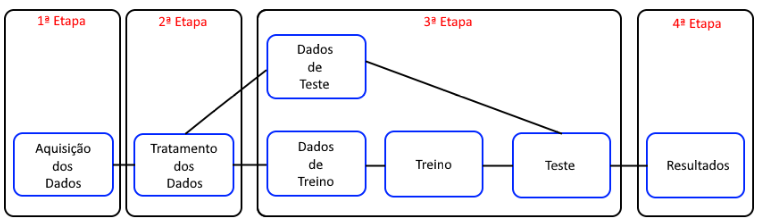
\includegraphics[width=1.\linewidth]{imagens/fluxograma.png}\\
  \end{center}
  \caption[Fluxograma do sistema proposto]{Fluxograma do sistema proposto}
  \label{fig:logo}
  %\legend{Fonte: Próprio Autor}
\end{figure}

\subsubsection{1ª Etapa - Aquisição dos dados}
	A primeira etapa envolve a escolha e a montagem de uma base de dados, algumas bases públicas estão disponíveis em https://www.football-data.co.uk e foram objetos de estudo em \citeonline{Ulmer2014}. Foram escolhidas deste mesmo site as seguintes bases de dados:
	\begin{itemize}
	\item Premier League (Temporada 2018/2019);
	\item Serie A (Temporada 2018/2019).
	\end{itemize}
	
	Foi escolhida também a base de dados do Brasileirão 2012 coletada do UOL Sports e disponível em https://github.com/zandree/statsBrazilianLeagueChampionship. Todas as bases estão no formato CSV.
	
	As bases da Premier League e Serie A foram feitas como cada linha sendo um jogo e esta linha possui os dados do time de casa e o time de fora. O resultado é dado como casa, empate ou fora. A base do Brasileirão tem sua construção diferente. Cada linha também é um jogo porém esta linha só possui os dados de um dos times, ou seja, cada jogo ocorrido terá 2 linhas uma para o time de casa e uma para o de fora. O resultado é dado com vitória, empate ou derrota.
	

\subsubsection{2ª Etapa - Tratamento dos dados}
	Esta etapa envolve todo o pré-processamento de dados. Primeiramente foi criado um DataFrame utilizando o Pandas para ler as bases de dados. A base da Premier League possui 380 linhas e 62 colunas enquanto a da Serie A possui 380 linhas e 61 colunas e ambas as bases não possuem dados faltantes. A base do Brasileirão possui 760 linhas, 50 colunas e 4 linhas com dados faltantes. As linhas com dados faltantes foram removidas e a base passou a ter 756 linhas.
	
	O próximo passo foi selecionar as características para a previsão. Nas bases Premier League e Serie A foram utilizadas as seguintes características:
	\begin{itemize}
	\item FTR - Resultado da partida (Casa, Empate, Fora);
	\item HS - Chutes do time da casa;
	\item AS - Chutes do time de fora;
	\item HST - Chutes do time da casa no alvo(gol);
	\item AST - Chutes do time de fora no alvo(gol);
	\item HF - Faltas cometidas pelo time da casa;
	\item AF - Faltas cometidas pelo time de fora;
	\item HC - Escanteios do time da casa;
	\item AC - Escanteios do time de fora;
	\item HY - Cartões Amarelos do time da casa;
	\item AY - Cartões Amarelos do time de fora;
	\item HR - Cartões Vermelhos do time da casa;
	\item AR - Cartões Vermelhos do time de fora;
	\item HTHG - Gols marcados pela equipe da casa até o intervalo;
	\item HTAG - Gols marcados pela equipe de fora até o intervalo.
	\end{itemize}
	
	Na base de dados do Brasileirão foram utilizadas as seguintes características:
	\begin{itemize}
	\item assistances - Assistências;
	\item receivedBalls - Bolas recebidas;
	\item recoveredBalls - Bolas recuperadas;
	\item lostBalls - Bolas perdidas;
	\item yellowCards - Cartões amarelos;
	\item redCards - Cartões vermelhos;
	\item receivedCrossBalls - Cruzamentos recebidos;
	\item missedCrossBalls - Cruzamentos perdidos;
	\item defenses - Defesas;
	\item sucessfulTackles - Desarmes com sucesso;
	\item unsucessfulTackles - Desarmes sem sucesso;
	\item sucessfulDribles - Dribles com sucesso;
	\item unsucessfulDribles - Dribles sem sucesso;
	\item givenCorners - Escanteios dados;
	\item receivedCorners - Escanteios recebidos;
	\item receivedFouls - Faltas recebidas;
	\item committedFouls - Faltas cometidas;
	\item goodFinishes - Boas finalizações;
	\item badFinishes - Finalizações ruins;
	\item ownGols - Gols marcados;
	\item offsides - Impedimentos;
	\item sucessfulLongPasses - Passes longos com sucesso;
	\item unsucessfulLongPasses - Passes longos sem sucesso;
	\item sucessfulPasses - Passes com sucesso;
	\item unsucessfulPasses - Passes sem sucesso;
	\item win - Vitória;
	\item draw - Empate;
	\item defeat - Derrota.
	\end{itemize}

	Em Premier League e Serie A os dados de FTR são categóricos e como FTR é o alvo da previsão foi preciso transformá-los para numéricos. Casa passou a ser 2, empate passou a ser 1 e fora passou a ser 0. No Brasileirão as características win, draw e defeat foram mescladas em uma só, chamada FTR, que também é o alvo da previsão, sendo 2 - vitória, 1 - empate e 0 - derrota.
	
	Com as características definidas o próximo passo foi padronizar os dados. Os dados foram padronizados com o \textit{StandardScaler} que está presente no Scikit-learn. O \textit{StandardScaler} transforma os dados de forma que sua distribuição tenha um valor médio de 0 e o desvio padrão 1. Cada valor no conjunto de dados será subtraído pela média das amostras e dividido pelo desvio padrão de todo o conjunto de dados \cite{StandardScaler}. O motivo da padronização foi para que classificadores como KNN possam performar melhor.
	
\subsubsection{3ª Etapa - Treino e teste}
	Foi definido qual era o alvo da previsão. Em todas as bases o alvo é a característica FTR a qual contém o resultado da partida. As demais características foram usadas para a previsão de FTR. Nesta etapa foram utilizados dois métodos diferentes de divisão de dados.
	
	O primeiro método foi o de divisão de treino e teste. Este método embaralha os dados e os divide em uma porcentagem para treino e outra para teste. Foi dividido 70\% para treino e 30\% para teste. A divisão dos dados gera quatro novos conjuntos de dados, sendo eles: características para treino, características para teste, alvo para treino e alvo para teste.
	
	O segundo método foi o de validação cruzada k-\textit{fold}. Neste método os dados de entrada são divididos em subconjuntos de dados k(chamados de \textit{folds}). O modelo é treinado com k-1 subconjuntos e depois avaliado no subconjunto que não foi utilizado para treinamento. O procedimento é repetido k vezes e em cada vez um subconjunto diferente é reservado para avaliação \cite{ValidacaoCruzada}. Foram utilizados 10 \textit{folds}.
	
	Para previsão dos resultados foram utilizadas diferentes abordagens. Foi feito a previsão com a base completa e com os dados do alvo agrupados de 2 em 2. Nas bases Premier League e Serie A foram feitas previsões com as seguintes abordagens:
	\begin{itemize}
	\item Casa, Empate e Fora;
	\item Casa e Fora;
	\item Casa e Empate;
	\item Fora e Empate.
	\end{itemize}
	
	Na base do Brasileirão as abordagens foram:
	\begin{itemize}
	\item Vitória, Empate e Derrota;
	\item Vitória e Derrota;
	\item Vitória e Empate;
	\item Derrota e Empate.
	\end{itemize}
	
	O próximo passo foi a criação dos modelos de previsão. Os classificadores utilizados foram:
	\begin{itemize}
	\item Regressão logística;
	\item Árvore de decisão;
	\item Floresta aleatória;
	\item K Nearest Neighbours(KNN);
	\item Support vector machine(SVM);
	\item Multi Layer Perceptron(MLP).
	\end{itemize}
	
	A regressão logística é uma técnica estatística que tem como objetivo modelar, a partir de um conjunto de observações, a relação “logística” entre uma variável resposta dicotômica e uma série de variáveis explicativas numéricas e/ou categóricas \cite{Isolete2013}. Define-se uma variável dependente (Y), ou variável de saída, e procura-se verificar a influência de uma ou mais variáveis ditas variáveis independentes (X’s) sobre esta variável dependente \cite{Zanini2007}. A regressão logística busca calcular ou prever a probabilidade da variável dependente assumir um determinado valor em função de outras variáveis. Regressão logística é um algoritmo de aprendizagem supervisionada.
	
	Árvores de decisão são modelos estatísticos para a classificação e previsão de dados. Formada por um conjunto de nós de decisão uma árvore começa com um nó, que se divide em possíveis resultados. Cada resultado leva a nós adicionais, que se ramificam em outras possibilidades. Uma árvore de decisão é essencialmente uma série de declarações if-elses, que quando aplicados a um registro de uma base de dados, resultam na classificação daquele registro \cite{Caraciolo2009}. Árvore de decisão é um algoritmo de aprendizagem supervisionada.
	
	Floresta aleatória é um classificador que consiste em uma combinação de árvores de decisão. Cada árvore depende dos valores de vetores aleatórios amostrados de forma independente e distribuídos igualmente para todas as árvores na floresta \cite{Breiman2001}. Uma floresta aleatória é construída por um simples voto de árvores de decisão usando o algoritmo Bagging. Todas as árvores treinadas são combinadas em uma composição com uma votação simples, usando o erro médio de todas as amostras \cite{DMITRIEVSKY2018}. Floresta aleatória é um algoritmo de aprendizagem supervisionada.
	
	K vizinhos mais próximos, do inglês \textit{K nearest neighbours(KNN)} é um algoritmo de aprendizagem supervisionada. O KNN classifica um elemento com base na proximidade de seus k vizinhos. O algoritmo calcula a distância do elemento alvo aos demais e as ordena da menor para o maior. Após ordenadas são selecionados apenas os k mais próximos vizinhos deste elemento alvo. Ele será classificado com as mesmas características do tipo de vizinho que está em maior quantidade dos k selecionados.
	
	Máquina de vetores de suporte, do inglês \textit{Support vector machine(SVM)} é um algoritmo de aprendizagem supervisionada, cujo objetivo é classificar determinado conjunto dados que são mapeados para um espaço de características multidimensional usando uma função kernel. Nela, o limite de decisão no espaço de entrada é representado por um hiperplano em dimensão superior no espaço \cite{Boser1992}. O que o SVM faz é encontrar um hiperplano entre dados de duas classes buscando maximizar a distância entre os pontos mais próximos em relação a cada uma das classes.
	
	Perceptron multicamadas, do inglês \textit{Multi Layer Perceptron(MLP)} é uma rede neural com camadas ocultas com um número indeterminado de neurônios. O MLP utiliza métodos derivados do gradiente no ajustes de seus pesos por retropropagação(\textit{backpropagation}). A rede consiste em uma camada de entrada, uma ou mais camadas escondidas e uma ou mais camadas de saída. Um sinal de entrada é propagado da entrada para saída e a saída propaga um sinal em caminho reverso alterando os pesos, para uma nova validação \cite{Amaral2014}.
	
	O scikit-learn possui todos esses classificadores. Para fazer a previsão primeiro é preciso instanciar o classificador, depois chamar a função de treino e ao final a função de previsão. Os modelos que serão apresentados a seguir valem para as 3 bases de dados. A abordagem a ser tratada é a da base de dados completa, a abordagem de 2 em 2 segue do mesmo raciocínio.
	
	Conforme a figura 2 a seguir, foi instanciado o classficador de regressão logística, depois chamada a função \textit{fit} responsável por treinar o modelo passando como parâmetro as características de treino e o alvo de treino. A função \textit{predict} é responsável pela previsão e nela é passada como parâmetro o alvo de teste, ou seja, com base no treinamento feito com as bases de treino o classificador vai tentar prever uma base ainda não vista, no caso a do alvo de teste.
	Todo esse procedimento foi feito com as bases do método de divisão 70-30. Para a validação cruzada é utilizado o \textit{cross\_val\_score} passando como parâmetros o classificador, o vetor de características, o alvo da previsão, e a quantidade de \textit{folds}.
	
\begin{figure}[htbp]
  \begin{center}
  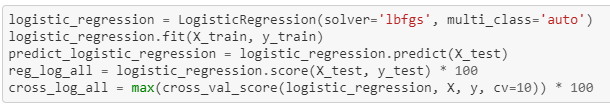
\includegraphics[width=1.\linewidth]{imagens/cod_reg_log.png}\\
  \end{center}
  \caption[Modelo de regressão logística]{Modelo de regressão logística}
  \label{fig:logo}
  %\legend{Fonte: Próprio Autor}
\end{figure}

	A árvore de decisão segue do mesmo raciocínio, conforme ilustrado na figura 3 a seguir.
	
\begin{figure}[htbp]
  \begin{center}
  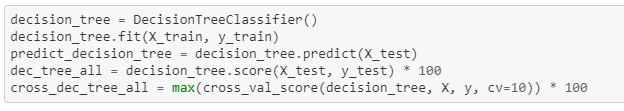
\includegraphics[width=1.\linewidth]{imagens/cod_dec_tree.png}\\
  \end{center}
  \caption[Modelo de árvore de decisão]{Modelo de árvore de decisão}
  \label{fig:logo}
  %\legend{Fonte: Próprio Autor}
\end{figure}

	Para os modelos de floresta aleatória e KNN é preciso definir o número de árvores para um e o número de vizinhos para o outro. A fim de encontrar qual o valor que gere a melhor previsão é feito um ``método cotovelo". Este método consiste em fazer previsões alterando os valores dentro de um intervalo. Ao terminar as previsões é feito a média das diferenças entre o valor previsto e o valor real e este valor é salvo em um vetor. O melhor número para utilizar é aquele que representa a menor diferença entre o valor real e o previsto. A floresta aleatória e o KNN seguem do mesmo raciocínio que os demais.
	
\begin{figure}[htbp]
  \begin{center}
  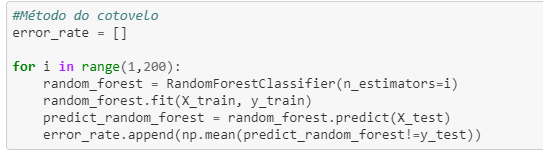
\includegraphics[width=0.8\linewidth]{imagens/cotovelo_floresta.png}\\
  \end{center}
  \caption[Método cotovelo floresta aleatória]{Método cotovelo floresta aleatória}
  \label{fig:logo}
  %\legend{Fonte: Próprio Autor}
\end{figure}

\begin{figure}[htbp]
  \begin{center}
  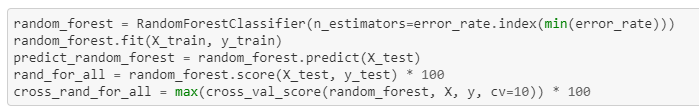
\includegraphics[width=1.\linewidth]{imagens/cod_rand_for.png}\\
  \end{center}
  \caption[Modelo de floresta aleatória]{Modelo de floresta aleatória}
  \label{fig:logo}
  %\legend{Fonte: Próprio Autor}
\end{figure}

\begin{figure}[htbp]
  \begin{center}
  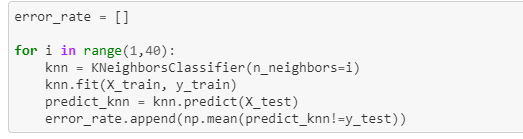
\includegraphics[width=0.8\linewidth]{imagens/cotovelo_knn.png}\\
  \end{center}
  \caption[Método cotovelo KNN]{Método cotovelo KNN}
  \label{fig:logo}
  %\legend{Fonte: Próprio Autor}
\end{figure}

\begin{figure}[htbp]
  \begin{center}
  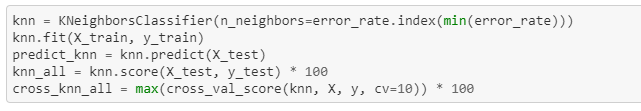
\includegraphics[width=1.\linewidth]{imagens/cod_knn.png}\\
  \end{center}
  \caption[Modelo KNN]{Modelo KNN}
  \label{fig:logo}
  %\legend{Fonte: Próprio Autor}
\end{figure}
	
	\break
	Para o modelo de SVM é utilizado o \textit{GridSearchCV}. O \textit{GridSearchCV} é um método onde é testado diferentes valores para alguns parâmetros do classificador a fim de descobrir qual combinação gera a melhor previsão. Primeiro é definido qual o classificador depois, uma lista com os parâmetros que vão ser testados e seus respectivos valores e a quantidade de \textit{folds}. Para o modelo de SVM não foi utilizado o método de divisão 70-30.
	
\begin{figure}[htbp]
  \begin{center}
  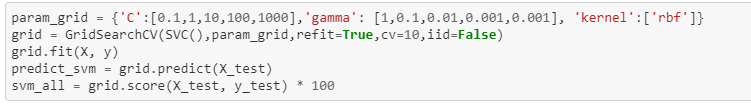
\includegraphics[width=1.\linewidth]{imagens/cod_svm.png}\\
  \end{center}
  \caption[Modelo SVM]{Modelo SVM}
  \label{fig:logo}
  %\legend{Fonte: Próprio Autor}
\end{figure}
	
	O modelo de MLP segue do mesmo raciocínio de regressão logística e árvore de decisão, conforme ilustrado na figura a seguir.
	
\begin{figure}[htbp]
  \begin{center}
  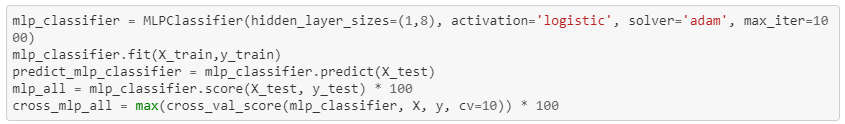
\includegraphics[width=1.\linewidth]{imagens/cod_mlp.png}\\
  \end{center}
  \caption[Modelo MLP]{Modelo MLP}
  \label{fig:logo}
  %\legend{Fonte: Próprio Autor}
\end{figure}

\subsubsection{4ª Etapa - Resultados}

	Para avaliar a precisão dos classificadores foi utilizado o método \textit{score} que esta contido em cada classificador. Este método retorna a acurácia ou o coeficiente de determinação de cada classificador. Os resultados obtidos foram:
	
\begin{figure}[htbp]
  \begin{center}
  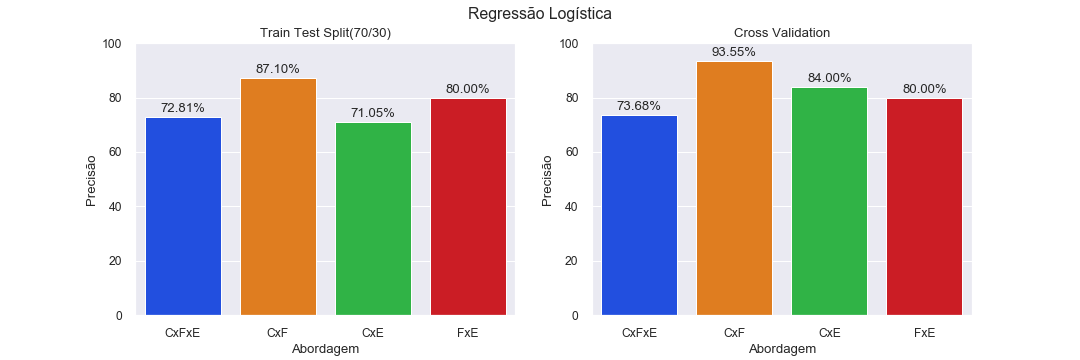
\includegraphics[width=1.05\linewidth]{imagens/resultados/regressao_logistica_pl.png}\\
  \end{center}
  \caption[Regressão logística Premier League]{Regressão logística Premier League}
  \label{fig:logo}
  %\legend{Fonte: Próprio Autor}
\end{figure}

\begin{figure}[htbp]
  \begin{center}
  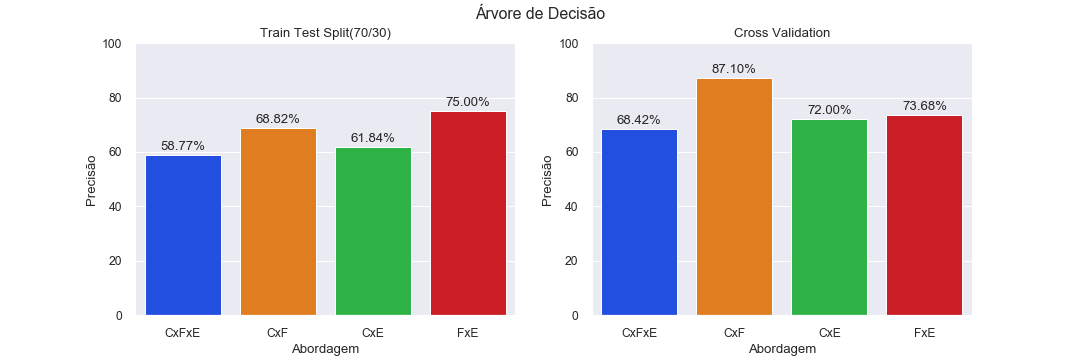
\includegraphics[width=1.05\linewidth]{imagens/resultados/arvore_decisao_pl.png}\\
  \end{center}
  \caption[Árvore de decisão Premier League]{Árvore de decisão Premier League}
  \label{fig:logo}
  %\legend{Fonte: Próprio Autor}
\end{figure}

\begin{figure}[htbp]
  \begin{center}
  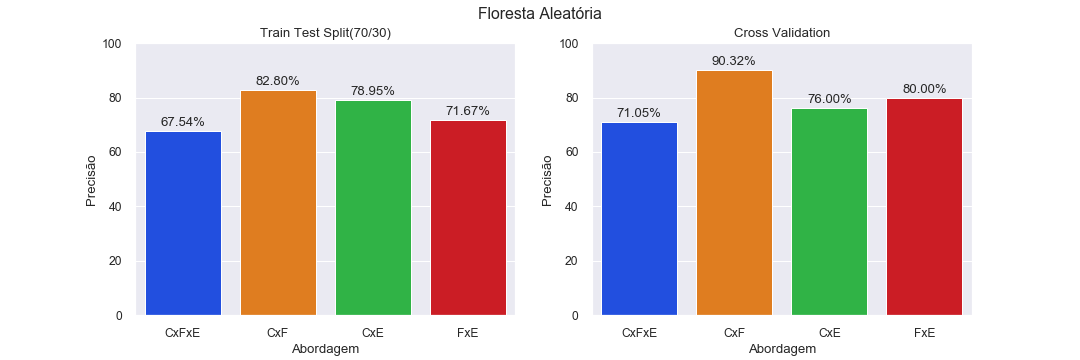
\includegraphics[width=1.05\linewidth]{imagens/resultados/floresta_aleatoria_pl.png}\\
  \end{center}
  \caption[Floresta aleatória Premier League]{Floresta aleatória Premier League}
  \label{fig:logo}
  %\legend{Fonte: Próprio Autor}
\end{figure}

\begin{figure}[htbp]
  \begin{center}
  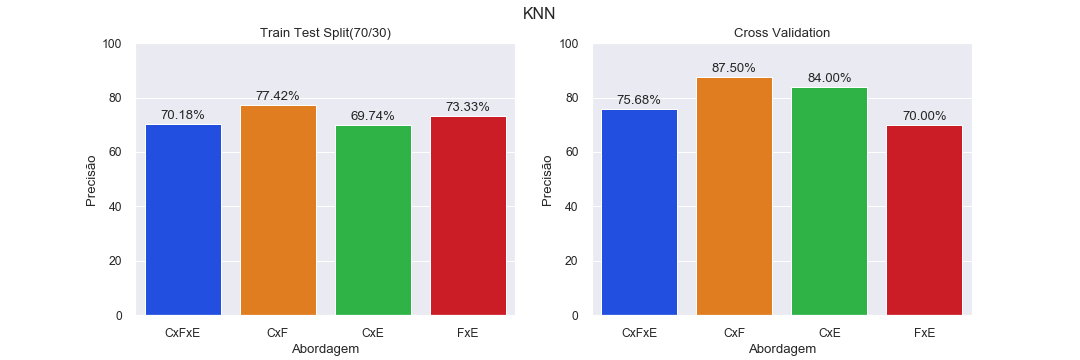
\includegraphics[width=1.05\linewidth]{imagens/resultados/knn_pl.png}\\
  \end{center}
  \caption[KNN Premier League]{KNN Premier League}
  \label{fig:logo}
  %\legend{Fonte: Próprio Autor}
\end{figure}

\begin{figure}[htbp]
  \begin{center}
  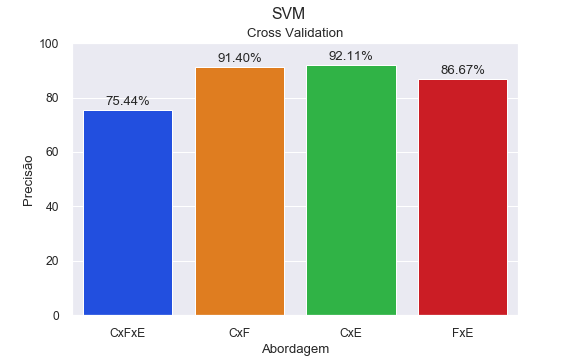
\includegraphics[width=0.7\linewidth]{imagens/resultados/svm_pl.png}\\
  \end{center}
  \caption[SVM Premier League]{SVM Premier League}
  \label{fig:logo}
  %\legend{Fonte: Próprio Autor}
\end{figure}

\begin{figure}[htbp]
  \begin{center}
  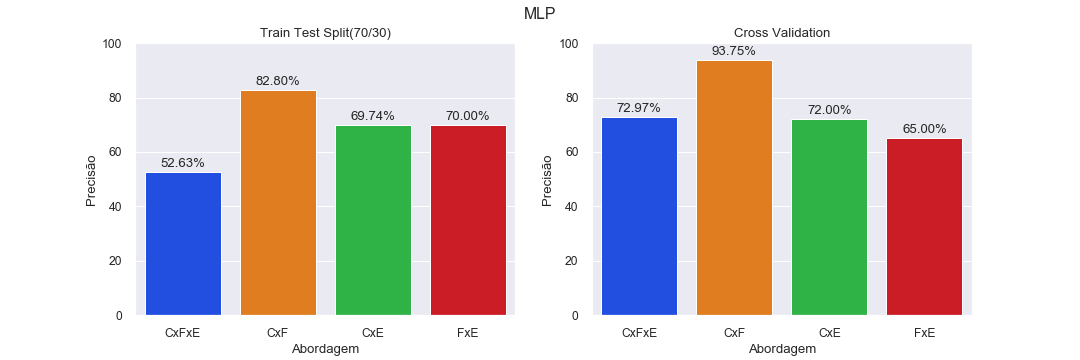
\includegraphics[width=1.05\linewidth]{imagens/resultados/mlp_pl.png}\\
  \end{center}
  \caption[MLP Premier League]{MLP Premier League}
  \label{fig:logo}
  %\legend{Fonte: Próprio Autor}
\end{figure}
	
\begin{figure}[htbp]
  \begin{center}
  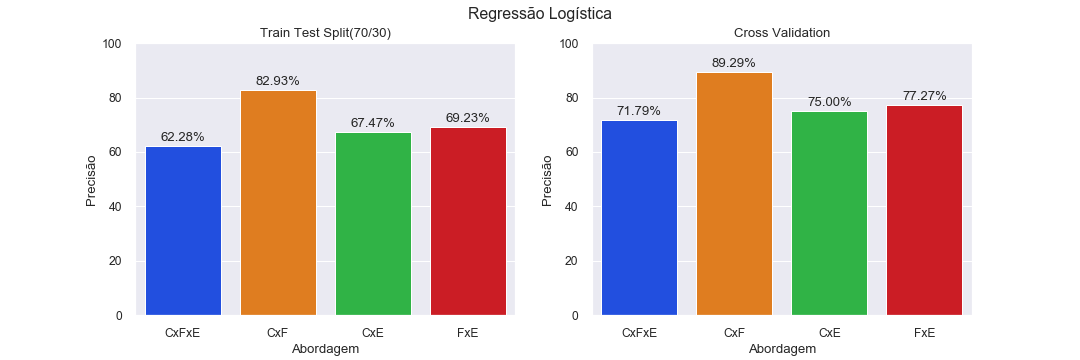
\includegraphics[width=1.05\linewidth]{imagens/resultados/regressao_logistica_sa.png}\\
  \end{center}
  \caption[Regressão logística Serie A]{Regressão logística Serie A}
  \label{fig:logo}
  %\legend{Fonte: Próprio Autor}
\end{figure}

\begin{figure}[htbp]
  \begin{center}
  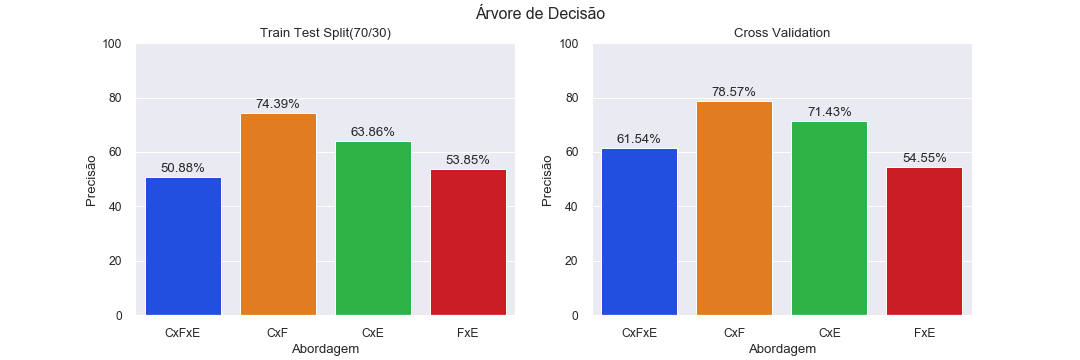
\includegraphics[width=1.05\linewidth]{imagens/resultados/arvore_decisao_sa.png}\\
  \end{center}
  \caption[Árvore de decisão Serie A]{Árvore de decisão Serie A}
  \label{fig:logo}
  %\legend{Fonte: Próprio Autor}
\end{figure}

\begin{figure}[htbp]
  \begin{center}
  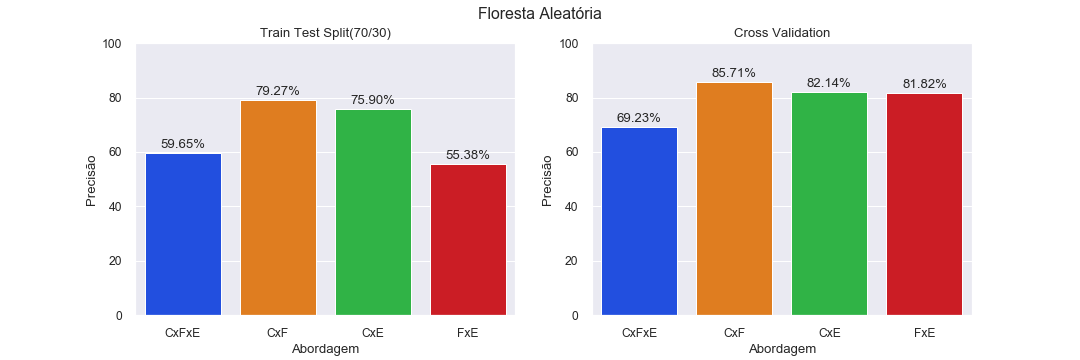
\includegraphics[width=1.05\linewidth]{imagens/resultados/floresta_aleatoria_sa.png}\\
  \end{center}
  \caption[Floresta aleatória Serie A]{Floresta aleatória Serie A}
  \label{fig:logo}
  %\legend{Fonte: Próprio Autor}
\end{figure}

\begin{figure}[htbp]
  \begin{center}
  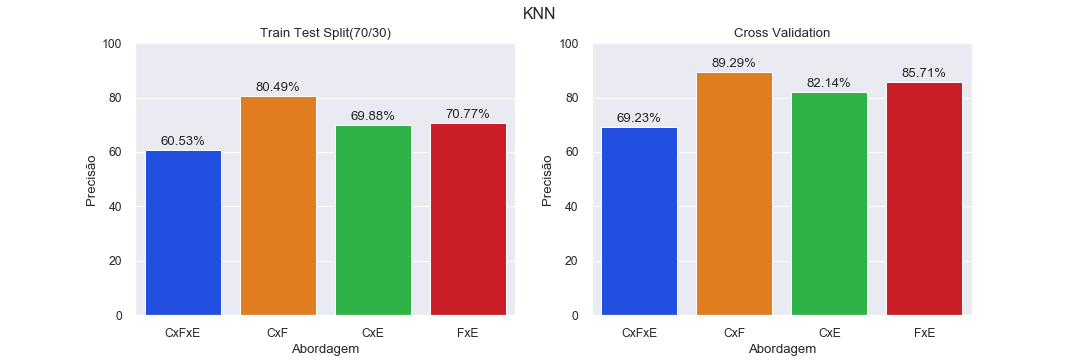
\includegraphics[width=1.05\linewidth]{imagens/resultados/knn_sa.png}\\
  \end{center}
  \caption[KNN Serie A]{KNN Serie A}
  \label{fig:logo}
  %\legend{Fonte: Próprio Autor}
\end{figure}

\begin{figure}[htbp]
  \begin{center}
  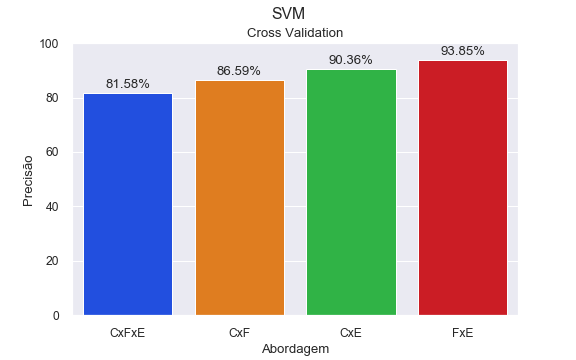
\includegraphics[width=0.7\linewidth]{imagens/resultados/svm_sa.png}\\
  \end{center}
  \caption[SVM Serie A]{SVM Serie A}
  \label{fig:logo}
  %\legend{Fonte: Próprio Autor}
\end{figure}

\begin{figure}[htbp]
  \begin{center}
  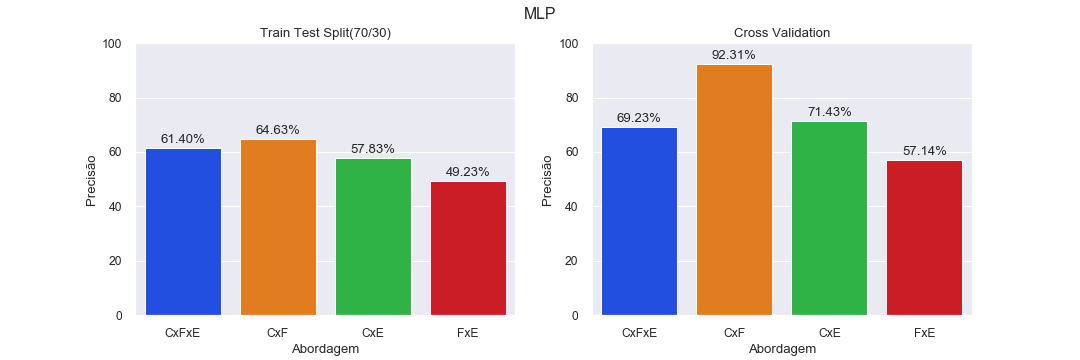
\includegraphics[width=1.05\linewidth]{imagens/resultados/mlp_sa.png}\\
  \end{center}
  \caption[MLP Serie A]{MLP Serie A}
  \label{fig:logo}
  %\legend{Fonte: Próprio Autor}
\end{figure}
	
\begin{figure}[htbp]
  \begin{center}
  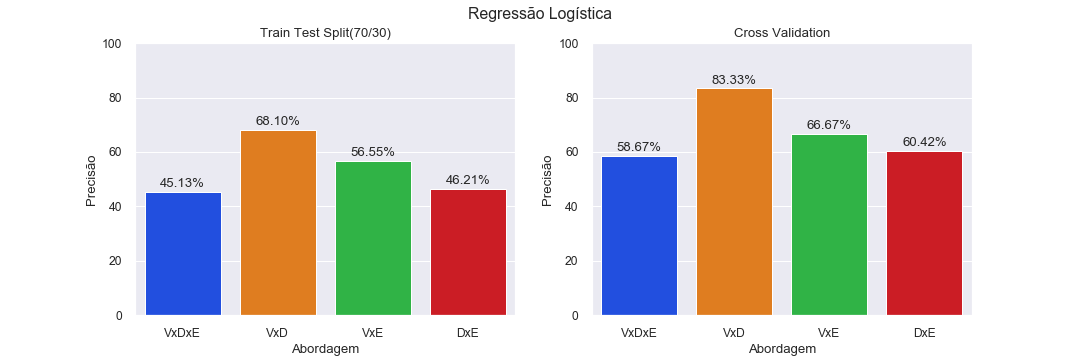
\includegraphics[width=1.05\linewidth]{imagens/resultados/regressao_logistica_br.png}\\
  \end{center}
  \caption[Regressão logística Brasileirão]{Regressão logística Brasileirão}
  \label{fig:logo}
  %\legend{Fonte: Próprio Autor}
\end{figure}

\begin{figure}[htbp]
  \begin{center}
  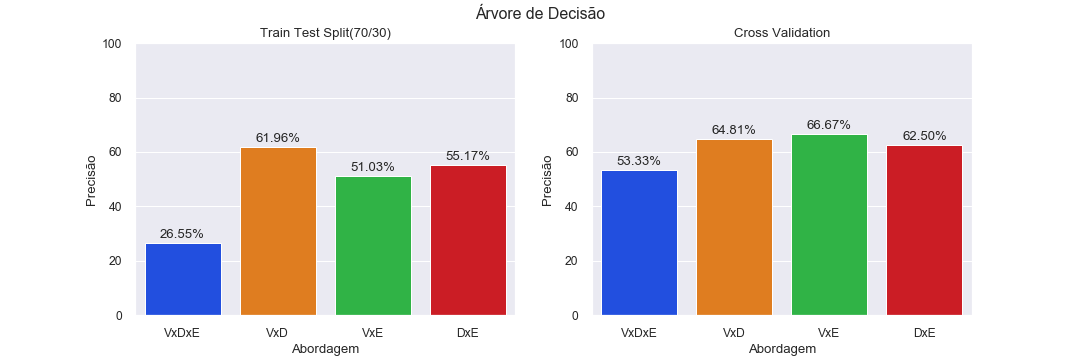
\includegraphics[width=1.05\linewidth]{imagens/resultados/arvore_decisao_br.png}\\
  \end{center}
  \caption[Árvore de decisão Brasileirão]{Árvore de decisão Brasileirão}
  \label{fig:logo}
  %\legend{Fonte: Próprio Autor}
\end{figure}

\begin{figure}[htbp]
  \begin{center}
  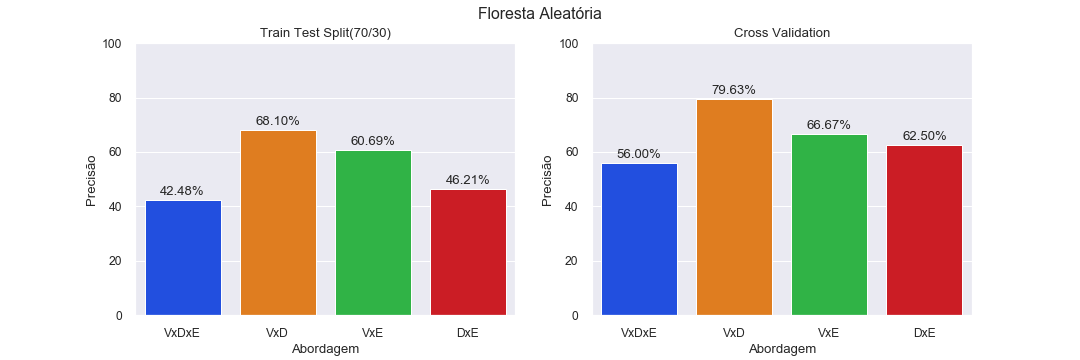
\includegraphics[width=1.05\linewidth]{imagens/resultados/floresta_aleatoria_br.png}\\
  \end{center}
  \caption[Floresta aleatória Brasileirão]{Floresta aleatória Brasileirão}
  \label{fig:logo}
  %\legend{Fonte: Próprio Autor}
\end{figure}

\begin{figure}[htbp]
  \begin{center}
  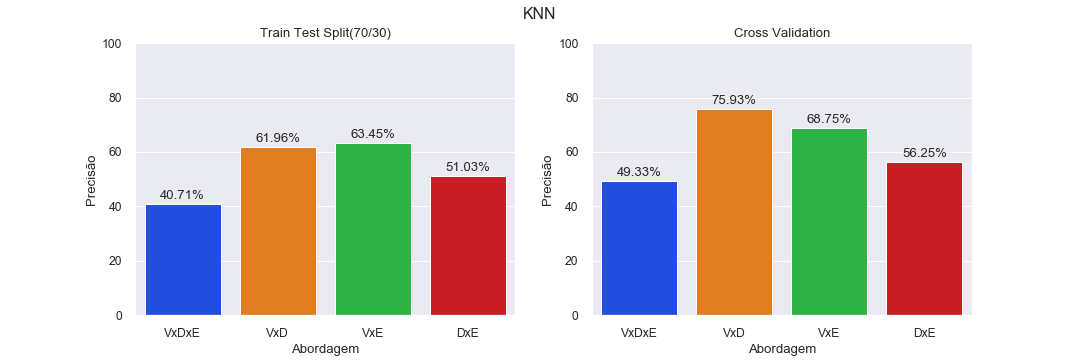
\includegraphics[width=1.05\linewidth]{imagens/resultados/knn_br.png}\\
  \end{center}
  \caption[KNN Brasileirão]{KNN Brasileirão}
  \label{fig:logo}
  %\legend{Fonte: Próprio Autor}
\end{figure}

\begin{figure}[htbp]
  \begin{center}
  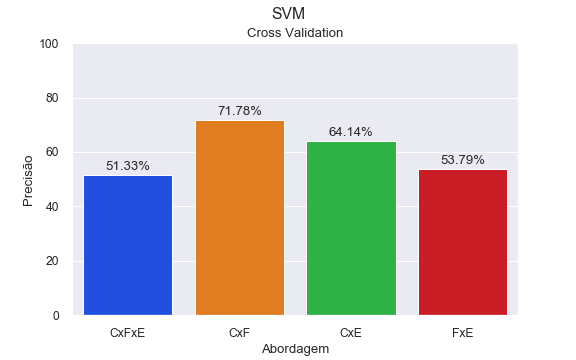
\includegraphics[width=0.7\linewidth]{imagens/resultados/svm_br.png}\\
  \end{center}
  \caption[SVM Brasileirão]{SVM Brasileirão}
  \label{fig:logo}
  %\legend{Fonte: Próprio Autor}
\end{figure}

\begin{figure}[htbp]
  \begin{center}
  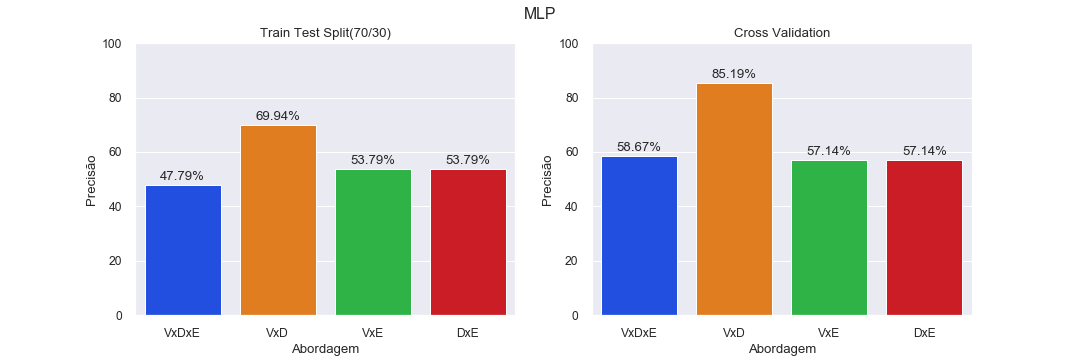
\includegraphics[width=1.05\linewidth]{imagens/resultados/mlp_br.png}\\
  \end{center}
  \caption[MLP Brasileirão]{MLP Brasileirão}
  \label{fig:logo}
  %\legend{Fonte: Próprio Autor}
\end{figure}	  
\break	
	
	
	
	
